\documentclass[]{article}
\usepackage{lmodern}
\usepackage{amssymb,amsmath}
\usepackage{ifxetex,ifluatex}
\usepackage{fixltx2e} % provides \textsubscript
\ifnum 0\ifxetex 1\fi\ifluatex 1\fi=0 % if pdftex
  \usepackage[T1]{fontenc}
  \usepackage[utf8]{inputenc}
\else % if luatex or xelatex
  \ifxetex
    \usepackage{mathspec}
  \else
    \usepackage{fontspec}
  \fi
  \defaultfontfeatures{Ligatures=TeX,Scale=MatchLowercase}
\fi
% use upquote if available, for straight quotes in verbatim environments
\IfFileExists{upquote.sty}{\usepackage{upquote}}{}
% use microtype if available
\IfFileExists{microtype.sty}{%
\usepackage{microtype}
\UseMicrotypeSet[protrusion]{basicmath} % disable protrusion for tt fonts
}{}
\usepackage[margin=1in]{geometry}
\usepackage{hyperref}
\hypersetup{unicode=true,
            pdftitle={finalRMarkdownDoc},
            pdfborder={0 0 0},
            breaklinks=true}
\urlstyle{same}  % don't use monospace font for urls
\usepackage{graphicx,grffile}
\makeatletter
\def\maxwidth{\ifdim\Gin@nat@width>\linewidth\linewidth\else\Gin@nat@width\fi}
\def\maxheight{\ifdim\Gin@nat@height>\textheight\textheight\else\Gin@nat@height\fi}
\makeatother
% Scale images if necessary, so that they will not overflow the page
% margins by default, and it is still possible to overwrite the defaults
% using explicit options in \includegraphics[width, height, ...]{}
\setkeys{Gin}{width=\maxwidth,height=\maxheight,keepaspectratio}
\IfFileExists{parskip.sty}{%
\usepackage{parskip}
}{% else
\setlength{\parindent}{0pt}
\setlength{\parskip}{6pt plus 2pt minus 1pt}
}
\setlength{\emergencystretch}{3em}  % prevent overfull lines
\providecommand{\tightlist}{%
  \setlength{\itemsep}{0pt}\setlength{\parskip}{0pt}}
\setcounter{secnumdepth}{0}
% Redefines (sub)paragraphs to behave more like sections
\ifx\paragraph\undefined\else
\let\oldparagraph\paragraph
\renewcommand{\paragraph}[1]{\oldparagraph{#1}\mbox{}}
\fi
\ifx\subparagraph\undefined\else
\let\oldsubparagraph\subparagraph
\renewcommand{\subparagraph}[1]{\oldsubparagraph{#1}\mbox{}}
\fi

%%% Use protect on footnotes to avoid problems with footnotes in titles
\let\rmarkdownfootnote\footnote%
\def\footnote{\protect\rmarkdownfootnote}

%%% Change title format to be more compact
\usepackage{titling}

% Create subtitle command for use in maketitle
\newcommand{\subtitle}[1]{
  \posttitle{
    \begin{center}\large#1\end{center}
    }
}

\setlength{\droptitle}{-2em}

  \title{finalRMarkdownDoc}
    \pretitle{\vspace{\droptitle}\centering\huge}
  \posttitle{\par}
    \author{}
    \preauthor{}\postauthor{}
    \date{}
    \predate{}\postdate{}
  

\begin{document}
\maketitle

Total Word Count: 2,986 Part 1: 585 Part 2: 573 Part 3: 1,828

Part 1

An attempt was made to produce identical choropleths of green roof (GR)
drainage area proportions by ward for Washington, DC using QGIS and R.
Since the products are similar, direct comparison of the processes used
and choropleths developed can be conducted. In QGIS and R, green roofs
were extracted from ``Best Management Practices'' (``BMP'') data by
querying on the ``Green\_Roof'' field (DCGISopendata, 2015). The
contributing drainage of these records was then summed, by ward, and
spatially joined with wards from ``Wards from 2012'' (``Wards'') data
(DCGISopendata, 2017). A new variable was then created to capture the
proportion of total drainage area within each ward. Finally, this
statistic was visualized using a graduated greens palette and projected
on OpenStreetMap basemaps. The choropleths indicate that ward 6 has the
greatest GR drainage area.

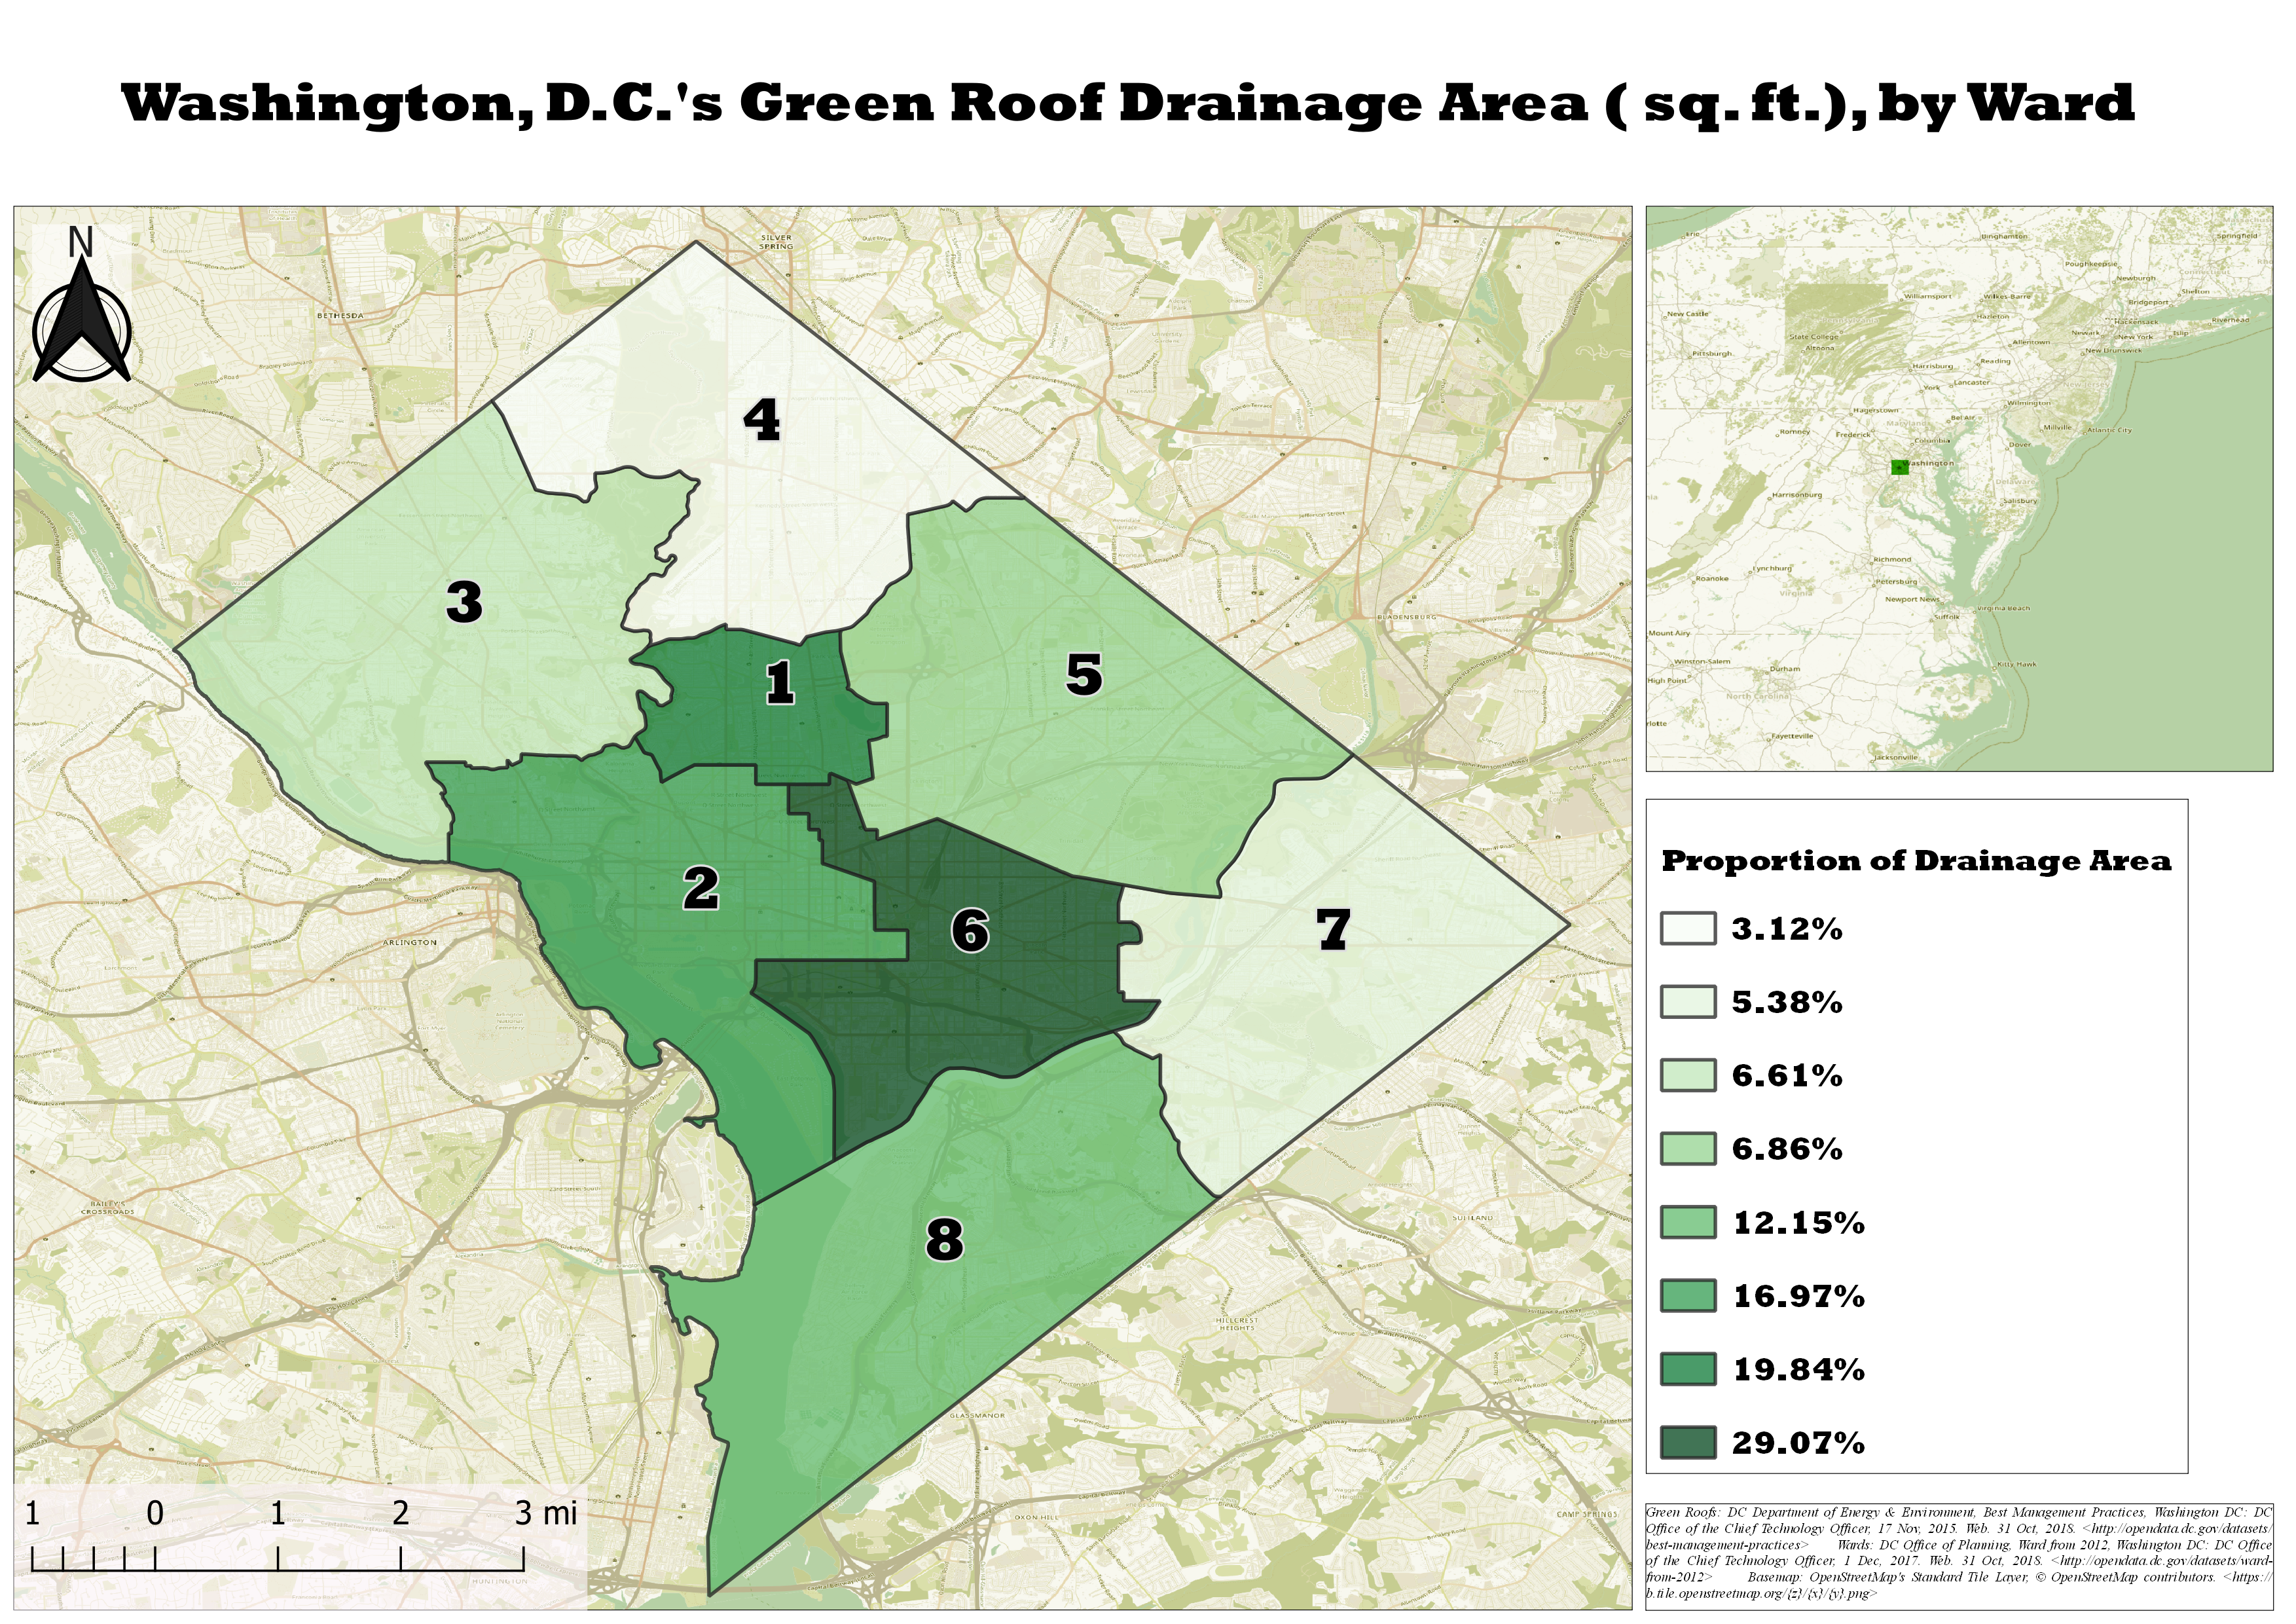
\includegraphics[width=48.71in]{1} While R and QGIS each have their
strengths, R seems more adequate for statistical analysis and handling
larger datasets is computationally cheaper. Combining this power with
libraries, R is undoubtedly superior at handling raw data. However, its
command-line nature means that the user must keep running the same lines
of code to visualize graphical alterations. Additionally, certain
features (fonts, scale-bar units, etc.) are not as customizable as in
QGIS. In contrast, QGIS's drag-and-drop GUI is much more interactive and
provides immediate visualization. One drawback of both GUIs and
command-line programs is the functionality of third-party libraries and
plug-ins. At best, the tools or code work with hiccups, but it is not
out of the ordinary for their functionality to be lost between version
updates.

\includegraphics[width=11.97in]{2} The choropleths produced rely on
``Wards'' data and ``BMP'' data that was compiled by the DC government.
As a result, the ``BMP'' data are three-years old and are likely missing
GRs. Likewise, there are redundant fields for ``BMP'' data and the
metadata do a poor job at describing variables. While OpenStreetMap
basemaps were used for context in both choropleths, this was notably
easier in R than in QGIS, as it failed to read some tile files. In
contrast, QGIS's map is far more visually appealing than R's. The
contextual second map and presence of a standalone legend direct the eye
around the page, which is preferable. The R choropleth causes the eye to
focus on the center of the image. While both maps are projected via
long-lat with a WGS84 datum and ellipsoid, the R map appears to have
stretched DC vertically. While the modifiable areal unit problem (MAUP)
would be an issue if the total GR drainage of each ward was visualized,
using proportion of drainage mitigates this (Openshaw, 1983). If the
unit of measure was changed, the proportion of drainage in ward 6 would
still be greater than all other wards. Furthermore, it is logical that
GR drainage should be represented by graduated shades of green, but this
poses an issue for the visually impaired. Nonetheless, because the
choropleths are overlaid on basemaps, which distinguish between the
areas of focus and context, the map is hopefully still readable. While
the use of graduated colors may verge on ``lying with maps'' (Monmonier,
2005, pp.~218-219), in that the variation of greens is not directly
proportionate to the difference in drainage proportions, it serves the
purpose of showing which wards have a disproportionate amount of
drainage. Overall, the final R product looks less jazzy (basic font,
reference position, etc.), and even though they are not perfect, the
choropleths serve their purpose: to show that wards 1, 2, and 6 contain
a disproportionate GR drainage area, relative to their overall size.

References DCGISopendata. (2015). ``Best Management Practices''. D.C.
Office of the Chief Technology Officer. Available at:
\url{http://opendata.dc.gov/datasets/best-management-practices}
DCGISopendata. (2017). ``Wards from 2012''. D.C. Office of the Chief
Technology Officer. Available at:
\url{http://opendata.dc.gov/datasets/ward-from-2012?geometry=-}
77.516\%2C38.707\%2C-76.512\%2C39.081 Monmonier, M. (2005). Lying with
Maps. Statistical Science, 20(3), pp.~215-222. Openshaw, S. (1983). The
Modifiable Areal Unit Problem. Norwick: Geo Books.

Part 2 Since ArcGIS was used, GeoJSON files required transformation to
Shapefiles before use in ArcGIS. Team Seven's data from 2016 was used.
QGIS was used to re-project all data into Shapefiles, using the BNG
(ESPG:27700). Re-projecting to BNG made for easy ArcGIS importation and
preserved distance measurements, for the UK. Point locations were
compiled using week seven's practical. Data for ``King's Cross'' was
corrected. City of London's wards were consolidated using the ``Merge''
function from the ``Editor Toolbar''. After this, the ``Join'' tool
wards data was joined to the polygons feature class.\\
1. Team Seven travelled approximately 46.604 kilometers on their
treasure hunt. This figure was calculated in a new field by calculating
geometry. Geometric property ``length'' was selected, with units set to
kilometers. The function measured the polyline with respect to BNG and
its unit of measure.\\
2. Team Seven passed within 100m of 24 stations on their hunt. To
compute this, the ``Buffer'' tool from the ``Geoprocessing'' toolbox was
used to generate a new polygon representing a 100m radius on the team's
route. ``Select By Location\ldots{}'' was used to select and count
stations intersecting the buffer.

\includegraphics[width=27.79in]{3} 3. The workflow of this solution is
methodologically similar to question two. ``Buffer'' was used to
generate a polygon representing a 300m buffer, then a ``Select By
Location\ldots{}'' query was used to highlight all point-locations
within 300m of the route. Statistics of the seventeen selected stations
show that their values sum to 62 points. It is worth noting that this
question and question two can be solved with less steps by using a
``Select By Location\ldots{}'' query to select points within a given
distance; however this alternative does not produce a visible buffer.

\includegraphics[width=25.85in]{4} 4. City of London has the greatest
male life expectancy at 84.31 and Weavers has the lowest at 75.06 years.
To compute these figures, ``Select By Location\ldots{}'' was utilized to
choose wards intersecting the route. Selected wards were then exported
as a new layer; the attribute table shows City of London, Weavers, and
their life expectancies.

\includegraphics[width=30.94in]{5} 5. Mean life expectancy for
intersected wards is 81.43 years. To compute this, wards' average life
expectancies were calculated from their respective male and female life
expectancies as a new field. Using ``Select By Location\ldots{}'', wards
intersecting the route were selected, and exported as a new layer. Using
this new layer, ``Statistics'' for average life expectancy were
generated to obtain the mean life expectancy for intersected wards.

\includegraphics[width=24.67in]{6} 6. According to quadrat analysis,
Ripley's K, and DBSCAN, the point locations are spatially clustered. To
start, wards and point locations were imported into R, since DBSCAN is
simpler to conduct than in ArcGIS, then a quadrat analysis was
conducted. This showed clustering more significant than a random Poisson
distribution would predict in 4 grids; however, this analysis suffers
greatly from issues of MAUP (Kwan, 2012). To address these drawbacks,
Ripley's K Test was conducted (Ripley, 1977, p.~172). It indicated that
as the test radius expanded, clustering became more significantly
significant; this is expected, but there

\includegraphics[width=11.17in]{7}

\includegraphics[width=11.17in]{8}

\includegraphics[width=11.17in]{9}

\includegraphics[width=11.17in]{10} References Ankerst, M., et al.
(1999). OPTICS: Ordering Points To Identify the Clustering Structure.
ACM SIGMOD International Conference on Management of Data. ACM Press,
pp.~49-60. Ester, M., et al. (1996). A density-based algorithm for
discovering clusters in large spatial databases with noise. Proceedings
of the Second International Conference on Knowledge Discovery and Data,
KDD-96, pp.~226-231.\\
Kwan, M-P. (2012). The Uncertain Geographic Context Problem. Annals of
the Association of American Geographers, 102(5), pp.~958-968. Savvas,
I.K., et al. (1967). A study of comparative clustering of EU countries
using the DBSCAN and k-means techniques within the theoretical framework
of systemic geopolitical analysis. International Journal of Grid and
Utility Computing, 8(2), pp. 94-108. Ohser, J. (1983). On estimators for
the reduced second moment measure of point processes. Series Statistics,
14(1), pp.~63-71. Ripley, B.D. (1977). Modelling Spatial Patterns.
Journal of the Royal Statistical Society, 39(2), pp.~172- 212.

Part 3

Creating and Implementing an ArcGIS Tool to Calculate
Herfindahl-Hirschman and Ellison-Glaeser Indices: A Case Study of
Supermarkets in Greater London Introduction Market concentration indices
are widely used to determine competition within a market for economic
evaluations, business transactions, and antitrust calculations. The
Herfindahl-Hirschman Index (HHI) is the most commonly used, as it
measures firm-level concentration. However, a drawback of HHI is that it
does not account for spatial concentration, and therefore discounts
agglomeration effects. The Ellison-Glaeser Index (EGI) addresses this
shortcoming by measuring market-level, location choice concentration,
while accounting for HHI. After consulting literature on benefits,
drawbacks and formulae of both indices, this paper will describe
implementation of a proposed ArcGIS tool that calculates HHI and EGI.
The tool's workflow will be described through its implementation in
calculating the two indices for supermarkets and groceries in Greater
London. Ultimately, the tool's functionality will be analyzed,
improvements and extensions will be suggested, and the concentration of
London's groceries will be visualized. 1---Literature Review
1.1---Herfindahl-Hirschman Index The HHI will be addressed first, as it
is used within EGI's calculations. It was theorized independently by
A.O. Hirschman (1945) and O.C. Herfindahl (1950), thus explaining the
hyphenated name (Board of Governors of the Federal Reserve System, 1993,
p.~188). Hirschman used the index to examine international supply market
concentration, while Herfindahl used it to analyze concentration in the
U.S. steel industry (Hirschman, 1945; Herfindahl, 1950). Today, HHI is
used in resource management, merger and acquisition evaluation, and
technological landscape appraisal (Scholz and Wellmer, 2013, pp.~14-25;
Cutler and Scott Morton, 2013, pp.~1964-1967; Liston-Heyes and
Pilkington, 2004, p.18). The index is considered reliable enough that
the U.S Federal Reserve uses it to analyze market concentrations and the
U.S. Department of Justice uses it to address competition and antitrust
cases (Board of Governors of the Federal Reserve System, 1993, p.~188;
Department of Justice and the Federal Trade Commission, 2010,
pp.~18-19). However, since HHI discounts markets' and firms' locations,
it is aspatial. Its metric should be considered an estimation of market
concentration that discounts spatiality. To calculate HHI, a defined
market, i, and the number of firms, N are required. Additionally, each
firm, j, must have a share, z\_j, of the market measure, say employment.
Firms' shares are squared and then summed, producing an HHI between zero
and one (Auvray and Agha, 2018, p.~4). Unconcentrated markets have
values below .15, highly concentrated markets have values .25 or above,
while those in between are moderately concentrated. Below, H indicates
the Herfindahl-Hirschman Index for the market area:
H=∑\emph{(j=1)\textsuperscript{N▒〖(z\_j)〗}2 1.2---Ellison-Glaeser
Index In 1994, Ellison and Glaeser developed their index to analyze
geographic concentration in U.S. manufacturing (Ellison and Glaeser,
1994). While it is less popular than HHI, this index explicitly
addresses spatiality by considering firms' locations (Auvray and Agha,
2018, p.~4). However, the measure is not directly comparable to HHI,
since it measures correlation of firms' location decisions. It is mainly
used by academics to examine agglomeration's effects (Lu and Tao, 2009,
p.~8; Lin et al., 2011, pp.~319-320; Yamamura and Goto, 2018,
pp.~445-446). In the model, N firms and M submarkets are used to measure
concentration of a market measure, say employment, for a market. Firms
sequentially choose to locate among the submarkets. Firm j's share of
market employment is z\_j. In submarket i, the industry's share of total
market employment is s\_i, while x\_i is the submarket's share of total
market employment:
γ=(∑}(i=1)\textsuperscript{M▒〖〖(s\_i-x\_i)〗}2-(1-∑\emph{(i=1)\textsuperscript{M▒〖〖x\_i〗}2)〗
∑}(j=1)\textsuperscript{N▒〖z\_j〗}2
〗)/((1-∑\emph{(i=1)\textsuperscript{M▒〖〖x\_i〗}2)(1-〗
∑}(j=1)\textsuperscript{N▒〖z\_j〗}2
))=(∑\emph{(i=1)\textsuperscript{M▒〖〖(s\_i-x\_i)〗}2-(1-∑}(i=1)\textsuperscript{M▒〖〖x\_i〗}2)〗
H〗)/((1-∑\_(i=1)\textsuperscript{M▒〖〖x\_i〗}2)(1-〗 H)) where H is
HHI for the market's industry (Ellison and Glaeser, 1994, pp.~12-13).
Product γ represents EGI. Positive results indicate correlation of
location choices, while negative products denote diffusion of location
choices. The proposed tool implements a simple EGI, whereas advanced
versions account for agglomeration effects (Casey and Smith, 2014,
pp.3-5). 1.3---Issues with Herfindahl-Hirschman and Ellison-Glaeser
Regardless of spatiality, the modifiable areal unit problem (MAUP)
affects both indices. MAUP results from areal unit choice and implies
that results for units with differing scales or shapes are inconsistent
(Jelinski and Wu, 1996, p.~130). Additionally, the checkboard problem
impacts EGI, as a result of it discounting areal unit adjacency. This
limits identification of agglomerations and spillovers to the areal unit
itself (Vignandi et al., 2016, p.~303). Regardless of these problems,
HHI and EGI are considered viable methods of estimating concentration,
but more robust indices have been developed and will be suggested in
section 4.2. 1.4---Comparison of HHI and EGI While both indices measure
market concentration, their indications differ. HHI illustrates
competition within an industry, whereas EGI indicates correlation among
firms' location decisions (Naude, 2006, pp.6-7). Therefore, HHI and EGI
should be considered together when analyzing industrial concentration,
but they are not directly comparable.\\
2---Motivation and Implementation of the Proposed Tool 2.1---Motivation
A concentration index tool for geographic information systems (GIS)
would serve a wide audience, primarily for the reasons outlined above.
It would allow users to quickly calculate and visualize both spatial and
aspatial indices. Considering Esri maintained near monopoly of the GIS
market in 2015, any tool should be tailored to ArcGIS (Esri, 2015). The
following sections briefly explore the proposed tool's parameters,
workflow, and implementation for major Greater London groceries'
employment---the metric of study.\\
2.2---Parameters Implementation requires three feature classes (FCs),
seven fields (as strings), and one output geodatabase. FCs denote
markets (polygon), submarkets of the markets (polygon), and firms
(point). Greater London's boroughs and wards will be considered markets
and submarkets, respectively, in this example. Firms are groceries. The
markets FC contains fields identifying markets and their employment. The
submarkets FC contains fields identifying the submarket, its market, and
its share of employment. The firms FC should contain fields denoting
firms and their employment. In the example, boroughs and wards will be
identified by their names and GSS Code, respectively. The output
geodatabase is populated by tool processes. 2.3---Workflow In Figure 1,
dark blue nodes indicate input FCs or geodatabases, celeste nodes
represent fields input as strings, gold nodes indicate processes, and
green nodes denote FCs or tables generated by processes. Connectors show
the workflow's direction. Numbers indicate order of processes. For
clarity, Table A lists processes' numbers, titles, and corresponding
PyScripts.

Figure 1---Workflow of the Proposed Tool

\includegraphics[width=19.79in]{11}

\includegraphics[width=17in]{12}

2.5---Example Data: London Groceries Locations for London groceries were
obtained from Geolytix (2018). Rough estimates of average employment per
store, per firm, were compiled (See groceryMarket.xlsx for details).
Wards, boroughs, and employment data were produced by London Datastore
(2015; 2018). City of London and Hackney are omitted due to insufficient
data. 2.4---Implementation The user runs the tool by double-clicking the
``Calculate HHI and EGI'' model inside the Concentration toolbox, inputs
required FCs and fields, and clicks ``OK''. For the purpose of this
paper, the model has been saved with the required fields and FCs from
the London groceries example; however, input can be altered for other
analyses. To avoid overwriting input FCs, the model initially duplicates
them as markets, submarkets, and firms in the output geodatabase (1).
From fields input as strings: markets contain markets and marketMetric;
submarkets contain submarkets, submarketMarket, and submarketMetric; and
firms contain firm and firmMetric. Beside joining indices to the input
markets FC, subsequent processes and outputs occur in the output
geodatabase. Following duplication, three FCs are created: markets are
spatially joined to firms (marketsJoinedToFirms) (2), submarkets are
spatially joined to markets (submarketsJoinedToMarkets) (3), and firms
are spatially joined to submarkets (firmsJoinedToSubmarkets) (4). For
EGI, marketsJoinedToFirms and submarketsJoinedToMarkets are used to
calculate industry HHIs for markets' firms by summing firms'
employments, by firm, by market. Proportions of firms' employment to
markets' industry employment are then calculated and squared. The sums
of squares represent HHIs for the industry, and are joined to
submarketsJoinedToMarkets, by market (5). Next,
submarketsJoinedToMarkets is used to calculate proportions of
submarkets' employment, relative to the total market, x\_i. These are
then squared, and summed, by market, giving
∑\emph{(i=1)\textsuperscript{M▒〖x\_i〗}2 . These figures are rejoined
to submarketsJoinedToMarkets (6). Subsequently,
submarketsJoinedToMarkets and firmsJoinedToSubmarkets are used to
calculate proportions of submarkets' industry employment relative to
market industry employment, s\_i. Next, x\_i is subtracted from s\_i.
The differences are squared and then summed, giving
∑}(i=1)\textsuperscript{M▒〖(s\_i-x\_i)〗}2 . These values are rejoined
to submarketsJoinedToMarkets, by market (7). The
submarketsJoinedToMarkets FC is then used to compute EGI, by market (8).
For HHI, sums of firms' employments, by market, are first calculated
with marketsJoinedToFirms (9). The resulting table's sums are rejoined
to marketsJoinedToFirms by market (10). Next, a concatenated
market\_firm field is calculated from market and firm fields so
firmMetric can be summed by both firm and market in process 13 (11).
Proportions of firm to market employment are then calculated (12). To
account for firms with multiple locations, proportions are summed by
market\_firm (13). These sums are squared (14) and a market field is
derived from market\_firm (15). Squared sums are then summed, by market,
to produce market HHIs (16), which are joined to the
submarketsJoinedToMarkets FC (17). Finally, HHIs and EGIs are joined to
the input markets feature class (18), allowing the user to visualize
results however she would like. There are notably fewer nodes for EGI
than HHI because EGI's contain more robust code. Code for EGI's
processes is shown in the Technical Appendix, while the rest can be
found in the accompanying folder.

3---Results Table B in the Appendix shows exact HHIs and EGIs for each
of the 31 boroughs modelled. Choropleth of Greater London Boroughs, by
Grocery Herfindahl-Hirschman Index

\includegraphics[width=23.69in]{13} Choropleth of Greater London
Boroughs, by Grocery Ellison-Glaeser Index

\includegraphics[width=23.56in]{14}

4---Discussion 4.3---London Groceries Example The tool appears to
accurately predict firm-level concentration with HHI; however, MAUP
seriously affects EGI via ward size variation. This compounds with a
lack of groceries in certain wards to bias estimates. For instance,
there are (supposedly) no groceries in seven of Bromley's twenty-two
wards. As a result, Bromley has the greatest choice diffusion of any
borough. Complete data and use of uniform submarket sizes, such as a
quadrat grid, would undoubtedly strengthen analyses. Likewise,
implementation of better-suited indices would address issues caused by
MAUP and the checkerboard problem. Grocery Distribution among Bromley's
Wards

\includegraphics[width=17.07in]{15} 4.1---Proposed Improvements for
Tool's Underlying Code While the tool calculates HHI and EGI, use of
functions in underlying code would decrease run-time and increase code
legibility. PyScripts should also address corner cases, as certain input
would likely ``break'' the tool. Improving validation procedures would
allow users to select fields instead of inputting them as strings.
Improvements would also allow model parameters to recognize visualized
layers or FCs, providing the option of selecting from populated dropdown
menus. Most importantly, HHI's PyScripts can be consolidated, so its
branch more closely resembles EGI's. Finally, the tool should allow the
user to select which indices are calculated. This selection would
decrease run-time and improve user experience. Ultimately, these
improvements would result in a more presentable workflow and a more
robust, quicker tool. 4.2---Proposed Improvements for Tool's Analytical
Capacity Even though using HHI and EGI in conjunction provides
sufficient estimation of concentration, more robust indices exist,
namely the Maurel-Sedillot, Guimarães, Marcon-Peuch, and
Duranton-Overman indices (Maurel and Sédillot, 1999; Guimarães et al.,
2011; Marcon and Peuch, 2014; Duranton and Overman, 2005). While MAUP
affects HHI and EGI, some of these indices address this issue, as well
as the checkerboard problem. Implementing Maurel-Sédillot could directly
address the issues affecting Bromley, in that it does not account for
submarket variations (Auvray-Agha, 2018, p.~5). Guimarães goes a step
further by spatially-weighting Ellison-Glaeser and Maurel-Sédillot
indices to addresses the checkerboard problem that affects both
(Guimarães et al., 2011). While Ellison-Glaeser and Maurel- Sédillot are
applicable for discrete submarkets and markets, Marcon-Peuch and
Duranton-Overman are continuous and account for interactions between
zones. Because of this, the MAUP and checkerboard issues are not a
problem. Furthermore, Marcon-Peuch examines absolute concentration of a
sector and denotes an industries concentration across the market, while
Duranton-Overman produces a relative measure that assigns greater weight
to the industry's overall presence in the market (Auvray-Agha, 2018,
pp.~3-6). While these indices all estimate concentration, they do so
over different scales, address different problems, and report different
concentration measures. Therefore, any exhaustive concentration tool
should allow the user to choose from possible indices, so that she can
calculate those that best suit her situation. 5---Conclusion The
proposed tool simplifies HHI and EGI analysis, but, with the suggested
improvements and extensions, it would be indispensable for analyzing
market concentrations. This endeavour has also demonstrated that, on
average, London groceries are concentrated at firm-level, but their
decisions of where to locate are not correlated. Subsequent research
should examine how use of a quadrat grid for defining submarkets,
instead of wards, impacts EGI measures. Furthermore, investigations
should determine if consumers are benefitting from firm-level
concentration or if antitrust action is warranted.

References Auvray, E. and Agha, S.B. (2018). ``Measuring geographic
concentration of economic activities''. 67th Annual Meeting of the
French Economic Association. Available at:
\url{https://afse2018.sciencesconf.org/190823/document} Board of
Governors of the Federal Reserve System. (1993). ``The
Herfindahl-Hirschman Index''. Federal Reserve Bank of St.~Louis.
Available at: \url{https://fraser.stlouisfed}
.org/files/docs/publications/FRB/pages/1990-1994/33101\_1990-1994.pdf
Casey, A.J. and Smith, B.O. (2014). ``Simulating confidence for the
Ellison-Glaeser index''. Journal of Urban Economics, 81, pp.~85-103.
Cutler, D.M. and Scott Morton, F. (2013). ``Hospitals, market share, and
consolidation''. Journal of the American Medical Association, 310(18),
pp.~1964-70. Department of Justice and the Federal Trade Commission.
(2010). ``Horizontal Merger Guidelines''. Department of Justice and the
Federal Trade Commission. Available at:
\url{https://www.justice.gov/sites/default/files/atr/legacy/2010/08/19/hmg-2010.pdf}
Duranton, G. and Overman, H.G. (2005). ``Testing for localization using
micro-geographic data''. The Review of Economic Studies, 72(4),
pp.~1077--1106. Ellison, G. and Glaeser, E. (1994). ``Geographic
Concentration in U.S. Manufacturing Industries: A Dartboard Approach''.
NBER Working Papers, No. 4840. Available at:
\url{https://www.nber.org/papers/w4840} Esri. (2015). ``Independent
Report Highlights Esri as Leader in Global GIS Market''. esri.com.
Available at:
\url{https://www.esri.com/esri-news/releases/15-1qtr/independent-}
report-highlights-esri-as-leader-in-global-gis-market {[}Accessed 30
December, 2018{]}. Geolytix. (2018). ``Retail Points: Supermarkets''.
Geolytix. \url{https://blog.geolytix.net/2018/10}
/23/4years-of-retail-points/ {[}Accessed 26 December, 2018{]}. Guimarães
et al. (2011). ``Accounting for Neighboring Effects in Measures of
Spatial Concentration''. Journal of Regional Science, 51(4),
pp.~678-693. Herfindahl, O.C. (1950). ``Concentration in the U.S. Steel
Industry''. Columbia University, Doctorate Dissertation. Hirschman, A.O.
(1945). National Power and the Structure of Foreign Trade. University of
California: Berkeley and Los Angeles. Jelinski, D.E. and Wu, J. (1996)
``The modifiable areal unit problem and implications for landscape
ecology'' Landscape Ecology, 11(3), pp.~129-140. Lin et al. (2011).
``Agglomeration and productivity: Firm-level evidence from China's
textile industry''. China Economic Review, 22(3), pp.~313-329.
Liston-Heyes, C and Pilkington A. (2004). ``Inventive concentration in
the production of green technology: A comparative analysis of fuel cell
patents''. Science and Public Policy, 31(1), pp.~15-25. London
Datastore. (2015). ``Ward Profiles and Atlases''. London Datastore.
\url{https://data.london.gov.uk/dataset} /ward-profiles-and-atlas
{[}Accessed 26 December 2018{]}. London Datastore. (2018). ``Statistical
GIS Boundary Files for London: London Wards 2014''. London Datastore.
\url{https://data.london.gov.uk/dataset/statistical-gis-boundary-}
files-london {[}Accessed 26 December, 2018{]}. Lu, J. and Tao, X.
(2007). ``Trends and Determinants of China's Industrial Agglomeration''.
Munich Personal RePEc Archive, No. 6597. Available at:
\url{https://mpra.ub.uni-} muenchen.de/6597/1/MPRA\_paper\_6597.pdf
Marcon, E. and Puech, F. (2014). ``Mesures de la concentration spatiale
en espace continue: théorie et applications''. Economie et statistique,
474(1), pp.~105--131. Maurel, F. and Sédillot, B. (1999) ``A measure of
the geographic concentration in French manufacturing industries''.
Regional Science and Urban Economics, 29(5), pp.~575 604. Naude, C.
(2006) ``Measures of Manufacturing Industry Concentration --
Implications for South Africa''. Development Policy Research Unit
Conference, 2006. Available at:
\url{http://citeseerx.ist.psu.edu/viewdoc/download?doi=10.1.1.485.3140\&rep=rep1\&type}=
pdf Scholz, R.W. and Wellmer, F.W. (2013). ``Approaching a dynamic view
on the availability of mineral resources: What we may learn from the
case of phosphorus?''. Global Environmental Change-Human and Policy
Dimensions, 23(1), pp.~11-27. Vignandi et al. (2016). ``Measures of
Industry Agglomeration in Brazil: a Study Addressing Neighboring
Effects'' Análise Econômica, 34(65), pp.~301-332. Yamamura, S. and Goto,
H. (2018). ``Location patterns and determinants of knowledge intensive
industries in the Tokyo Metropolitan Area''. Japan Architectural Review,
1(4), pp.~443-456. Appendix

\includegraphics[width=13.97in]{16}

Technical Appendix Process 5---Calculate Market Industry HHI
\#-------------------------------------------------------------------------------
\# Name: calcMarketIndustryHHI \# \# Purpose: calculate industry HHI for
a market \# \# Use markets joined to firms to sum firm metric by firm,
by \# market-firm metric; \# Use markets joined to firms to sum firm
metric by market- \# market industry metic; \# Join market industry
metric to the table resulting from the sum \# of firm metric by firm, by
market; \# Calculate the proportion of firm metric to market industry \#
metric - Zj; \# Calculate the square of Zj; \# Sum Zj squared, by market
- market industry HHI; \# Join market industry HHI to submarkets to
markets spatial join; \# \# Author: Matthew Sutton \# \# Created:
29/12/2018
\#-------------------------------------------------------------------------------
import arcpy

\section{get and set marketsJoinedToFirms, markets, and
submarkets}\label{get-and-set-marketsjoinedtofirms-markets-and-submarkets}

marketsJoinedToFirms = arcpy.GetParameterAsText(0)
submarketsToMarketsJoin = arcpy.GetParameterAsText(1)
\#\#\#\#\#\#\#\#\#\#\#\#\#\#\#\#\#\#\#\#\#\#\#\#\#\#\#\#\#\#\#\#\#\#\#\#\#\#\#\#\#\#\#\#\#\#\#\#\#\#\#\#\#\#\#\#\#\#\#\#\#\#\#\#\#\#\#\#\#\#\#\#\#\#\#\#\#\#\#
\#\#\#\#\#\#\#\#\#\#\#\#\#\#\#\#\#\#\#\#\#\#\#\#\#\#\#\#\#\#\#\#\#\#\#\#\#\#\#\#\#\#\#\#\#\#\#\#\#\#\#\#\#\#\#\#\#\#\#\#\#\#\#\#\#\#\#\#\#\#\#\#\#\#\#\#\#\#\#
\#\#\#\#\#\#\#\#\#\#\#\#\#\#\#\#\#\#\#\#\#\#\#\#\#\#\#\#\#\#\#\#\#\#\#\#\#\#\#\#\#\#\#\#\#\#\#\#\#\#\#\#\#\#\#\#\#\#\#\#\#\#\#\#\#\#\#\#\#\#\#\#\#\#\#\#\#\#\#
\#Use markets joined to firms to sum firm metic by firm by market-firm
\#metic; \#get path from marketsJoinedToFirms and create output table
path in its \#geodatabase marketsJoinedToFirmsPath =
{[}marketsJoinedToFirms{]} wantedPathList =
marketsJoinedToFirmsPath{[}0{]}.split(`\textbackslash{}')
wantedPathList.pop(-1) path = wantedPathList{[}0{]} index = 1 while
index \textless{} len(wantedPathList): path = path +
``\textbackslash{}'' + wantedPathList{[}index{]} index = index + 1
sumFirmMetricByFirmByMarketPath = str(path) +
``\textbackslash{}sumFirmMetricByFirmByMarket''

\section{delete sumFirmMetricByFirmByMarket table if it already
exists}\label{delete-sumfirmmetricbyfirmbymarket-table-if-it-already-exists}

if arcpy.Exists(sumFirmMetricByFirmByMarketPath):
arcpy.Delete\_management(sumFirmMetricByFirmByMarketPath)

\section{sum firms' metric by firm by
market}\label{sum-firms-metric-by-firm-by-market}

arcpy.Statistics\_analysis (marketsJoinedToFirms,
sumFirmMetricByFirmByMarketPath, {[}{[}``firmMetric'', ``SUM''{]}{]},
{[}``firm'',``market''{]})

\section{rename summed metric field}\label{rename-summed-metric-field}

arcpy.AlterField\_management (sumFirmMetricByFirmByMarketPath,
``SUM\_firmMetric'', ``firmMetricByFirmByMarket'',
``firmMetricByFirmByMarket'')
\#\#\#\#\#\#\#\#\#\#\#\#\#\#\#\#\#\#\#\#\#\#\#\#\#\#\#\#\#\#\#\#\#\#\#\#\#\#\#\#\#\#\#\#\#\#\#\#\#\#\#\#\#\#\#\#\#\#\#\#\#\#\#\#\#\#\#\#\#\#\#\#\#\#\#\#\#\#\#
\#\#\#\#\#\#\#\#\#\#\#\#\#\#\#\#\#\#\#\#\#\#\#\#\#\#\#\#\#\#\#\#\#\#\#\#\#\#\#\#\#\#\#\#\#\#\#\#\#\#\#\#\#\#\#\#\#\#\#\#\#\#\#\#\#\#\#\#\#\#\#\#\#\#\#\#\#\#\#
\#\#\#\#\#\#\#\#\#\#\#\#\#\#\#\#\#\#\#\#\#\#\#\#\#\#\#\#\#\#\#\#\#\#\#\#\#\#\#\#\#\#\#\#\#\#\#\#\#\#\#\#\#\#\#\#\#\#\#\#\#\#\#\#\#\#\#\#\#\#\#\#\#\#\#\#\#\#\#
\#Use markets joined to firms to sum firm metric by market - market
industry \#metric; \#set table name sumFirmMetricByMarketPath =
str(path) + ``\textbackslash{}sumFirmMetricByMarket''

\section{delete sumFirmMetricByMarket table if it already
exists}\label{delete-sumfirmmetricbymarket-table-if-it-already-exists}

if arcpy.Exists(sumFirmMetricByMarketPath):
arcpy.Delete\_management(sumFirmMetricByMarketPath)

\section{sum firms' metric by market}\label{sum-firms-metric-by-market}

arcpy.Statistics\_analysis (marketsJoinedToFirms,
sumFirmMetricByMarketPath, {[}{[}``firmMetric'', ``SUM''{]}{]},
{[}``market''{]})

\section{rename summed metric field}\label{rename-summed-metric-field-1}

arcpy.AlterField\_management (sumFirmMetricByMarketPath,
``SUM\_firmMetric'', ``firmMetricByMarket'', ``firmMetricByMarket'')
\#\#\#\#\#\#\#\#\#\#\#\#\#\#\#\#\#\#\#\#\#\#\#\#\#\#\#\#\#\#\#\#\#\#\#\#\#\#\#\#\#\#\#\#\#\#\#\#\#\#\#\#\#\#\#\#\#\#\#\#\#\#\#\#\#\#\#\#\#\#\#\#\#\#\#\#\#\#\#
\#\#\#\#\#\#\#\#\#\#\#\#\#\#\#\#\#\#\#\#\#\#\#\#\#\#\#\#\#\#\#\#\#\#\#\#\#\#\#\#\#\#\#\#\#\#\#\#\#\#\#\#\#\#\#\#\#\#\#\#\#\#\#\#\#\#\#\#\#\#\#\#\#\#\#\#\#\#\#
\#\#\#\#\#\#\#\#\#\#\#\#\#\#\#\#\#\#\#\#\#\#\#\#\#\#\#\#\#\#\#\#\#\#\#\#\#\#\#\#\#\#\#\#\#\#\#\#\#\#\#\#\#\#\#\#\#\#\#\#\#\#\#\#\#\#\#\#\#\#\#\#\#\#\#\#\#\#\#
\#Join market industry metric to firmMetricByFirmByMarket table by
market

\section{delete firmMetricByFirmByMarket field if it exists in
marketsJoinedToFirms}\label{delete-firmmetricbyfirmbymarket-field-if-it-exists-in-marketsjoinedtofirms}

if len(arcpy.ListFields(sumFirmMetricByFirmByMarketPath,
``firmMetricByMarket'')) \textgreater{} 0:
arcpy.DeleteField\_management(sumFirmMetricByFirmByMarketPath,{[}``firmMetricByMarket''{]})

\section{join the firmMetricByMarket to sumFirmMetricByFirmByMarket
table by
market}\label{join-the-firmmetricbymarket-to-sumfirmmetricbyfirmbymarket-table-by-market}

arcpy.JoinField\_management (sumFirmMetricByFirmByMarketPath,
``market'', sumFirmMetricByMarketPath, ``market'',
{[}``firmMetricByMarket''{]})
\#\#\#\#\#\#\#\#\#\#\#\#\#\#\#\#\#\#\#\#\#\#\#\#\#\#\#\#\#\#\#\#\#\#\#\#\#\#\#\#\#\#\#\#\#\#\#\#\#\#\#\#\#\#\#\#\#\#\#\#\#\#\#\#\#\#\#\#\#\#\#\#\#\#\#\#\#\#\#
\#\#\#\#\#\#\#\#\#\#\#\#\#\#\#\#\#\#\#\#\#\#\#\#\#\#\#\#\#\#\#\#\#\#\#\#\#\#\#\#\#\#\#\#\#\#\#\#\#\#\#\#\#\#\#\#\#\#\#\#\#\#\#\#\#\#\#\#\#\#\#\#\#\#\#\#\#\#\#
\#\#\#\#\#\#\#\#\#\#\#\#\#\#\#\#\#\#\#\#\#\#\#\#\#\#\#\#\#\#\#\#\#\#\#\#\#\#\#\#\#\#\#\#\#\#\#\#\#\#\#\#\#\#\#\#\#\#\#\#\#\#\#\#\#\#\#\#\#\#\#\#\#\#\#\#\#\#\#
\#Calculate the proportion of firm metric to market industry metric -
Zj; \#add Zj field to sumFirmMetricByFirmByMarket table
arcpy.AddField\_management (sumFirmMetricByFirmByMarketPath, ``Zj'',
``FLOAT'', 15, 14)

\section{set to calculate proportion of firm metric to total market
industry
metric}\label{set-to-calculate-proportion-of-firm-metric-to-total-market-industry-metric}

calculateProp = ``!firmMetricByFirmByMarket!/!firmMetricByMarket!''

\section{calculate Zj}\label{calculate-zj}

arcpy.CalculateField\_management (sumFirmMetricByFirmByMarketPath,
``Zj'', calculateProp, ``PYTHON\_9.3'')
\#\#\#\#\#\#\#\#\#\#\#\#\#\#\#\#\#\#\#\#\#\#\#\#\#\#\#\#\#\#\#\#\#\#\#\#\#\#\#\#\#\#\#\#\#\#\#\#\#\#\#\#\#\#\#\#\#\#\#\#\#\#\#\#\#\#\#\#\#\#\#\#\#\#\#\#\#\#\#
\#\#\#\#\#\#\#\#\#\#\#\#\#\#\#\#\#\#\#\#\#\#\#\#\#\#\#\#\#\#\#\#\#\#\#\#\#\#\#\#\#\#\#\#\#\#\#\#\#\#\#\#\#\#\#\#\#\#\#\#\#\#\#\#\#\#\#\#\#\#\#\#\#\#\#\#\#\#\#
\#\#\#\#\#\#\#\#\#\#\#\#\#\#\#\#\#\#\#\#\#\#\#\#\#\#\#\#\#\#\#\#\#\#\#\#\#\#\#\#\#\#\#\#\#\#\#\#\#\#\#\#\#\#\#\#\#\#\#\#\#\#\#\#\#\#\#\#\#\#\#\#\#\#\#\#\#\#\#
\#Calculate the square of Zj; \#add ZjSquared field to
sumFirmMetricByFirmByMarket table arcpy.AddField\_management
(sumFirmMetricByFirmByMarketPath, ``ZjSquared'', ``FLOAT'', 15, 14)

\section{set to calculate square of
Zj}\label{set-to-calculate-square-of-zj}

calculateSquare = ``!Zj!*!Zj!"

\section{calculate square of Zj}\label{calculate-square-of-zj}

arcpy.CalculateField\_management (sumFirmMetricByFirmByMarketPath,
``ZjSquared'', calculateSquare, ``PYTHON\_9.3'')
\#\#\#\#\#\#\#\#\#\#\#\#\#\#\#\#\#\#\#\#\#\#\#\#\#\#\#\#\#\#\#\#\#\#\#\#\#\#\#\#\#\#\#\#\#\#\#\#\#\#\#\#\#\#\#\#\#\#\#\#\#\#\#\#\#\#\#\#\#\#\#\#\#\#\#\#\#\#\#
\#\#\#\#\#\#\#\#\#\#\#\#\#\#\#\#\#\#\#\#\#\#\#\#\#\#\#\#\#\#\#\#\#\#\#\#\#\#\#\#\#\#\#\#\#\#\#\#\#\#\#\#\#\#\#\#\#\#\#\#\#\#\#\#\#\#\#\#\#\#\#\#\#\#\#\#\#\#\#
\#\#\#\#\#\#\#\#\#\#\#\#\#\#\#\#\#\#\#\#\#\#\#\#\#\#\#\#\#\#\#\#\#\#\#\#\#\#\#\#\#\#\#\#\#\#\#\#\#\#\#\#\#\#\#\#\#\#\#\#\#\#\#\#\#\#\#\#\#\#\#\#\#\#\#\#\#\#\#
\#Sum Zj squared, by market - market industry HHI; \#set table name
marketIndustryHHIPath = str(path) +
``\textbackslash{}marketIndustryHHI''

\section{delete marketIndustryHHI table if it already
exists}\label{delete-marketindustryhhi-table-if-it-already-exists}

if arcpy.Exists(marketIndustryHHIPath):
arcpy.Delete\_management(marketIndustryHHIPath)

\section{sum firms' metric by
market}\label{sum-firms-metric-by-market-1}

arcpy.Statistics\_analysis (sumFirmMetricByFirmByMarketPath,
marketIndustryHHIPath, {[}{[}``ZjSquared'', ``SUM''{]}{]},
{[}``market''{]})

\section{rename summed metric field}\label{rename-summed-metric-field-2}

arcpy.AlterField\_management (marketIndustryHHIPath, ``SUM\_ZjSquared'',
``marketIndustryHHI'', ``marketIndustryHHI'')
\#\#\#\#\#\#\#\#\#\#\#\#\#\#\#\#\#\#\#\#\#\#\#\#\#\#\#\#\#\#\#\#\#\#\#\#\#\#\#\#\#\#\#\#\#\#\#\#\#\#\#\#\#\#\#\#\#\#\#\#\#\#\#\#\#\#\#\#\#\#\#\#\#\#\#\#\#\#\#
\#\#\#\#\#\#\#\#\#\#\#\#\#\#\#\#\#\#\#\#\#\#\#\#\#\#\#\#\#\#\#\#\#\#\#\#\#\#\#\#\#\#\#\#\#\#\#\#\#\#\#\#\#\#\#\#\#\#\#\#\#\#\#\#\#\#\#\#\#\#\#\#\#\#\#\#\#\#\#
\#\#\#\#\#\#\#\#\#\#\#\#\#\#\#\#\#\#\#\#\#\#\#\#\#\#\#\#\#\#\#\#\#\#\#\#\#\#\#\#\#\#\#\#\#\#\#\#\#\#\#\#\#\#\#\#\#\#\#\#\#\#\#\#\#\#\#\#\#\#\#\#\#\#\#\#\#\#\#
\#Join market industry HHI to submarkets to markets spatial join;
\#delete firmMetricByFirmByMarket field if it exists in
marketsJoinedToFirms if len(arcpy.ListFields(submarketsToMarketsJoin,
``marketIndustryHHI'')) \textgreater{} 0:
arcpy.DeleteField\_management(submarketsToMarketsJoin,{[}``marketIndustryHHI''{]})

\section{join marketIndustryHHI to submarketsToMarketsJoin by
market}\label{join-marketindustryhhi-to-submarketstomarketsjoin-by-market}

arcpy.JoinField\_management (submarketsToMarketsJoin, ``market'',
marketIndustryHHIPath, ``market'', {[}``marketIndustryHHI''{]})

arcpy.SetParameterAsText(2,submarketsToMarketsJoin)

Process 6---Calculate Xi and Sum of Xi Squared by Market
\#-------------------------------------------------------------------------------
\# Name: calcXiAndSumOfXiSquaredByMarket \# Purpose: Calculate Xi: \# \#
Calculate the proportion of total submarket metric to total \# market
metric - Xi; \# Calculate the square of Xi - Xi squared; \# Sum squared
Xi by market; \# Rejoin sum of square Xi's to spatial join of submarkets
to \# markets by market \# \# Author: Matthew Sutton \# \# Created:
29/12/2018
\#-------------------------------------------------------------------------------
import arcpy

\section{get and set
submarketsJoinedToMarkets}\label{get-and-set-submarketsjoinedtomarkets}

submarketsJoinedToMarkets = arcpy.GetParameterAsText(0)
\#\#\#\#\#\#\#\#\#\#\#\#\#\#\#\#\#\#\#\#\#\#\#\#\#\#\#\#\#\#\#\#\#\#\#\#\#\#\#\#\#\#\#\#\#\#\#\#\#\#\#\#\#\#\#\#\#\#\#\#\#\#\#\#\#\#\#\#\#\#\#\#\#\#\#\#\#\#\#
\#\#\#\#\#\#\#\#\#\#\#\#\#\#\#\#\#\#\#\#\#\#\#\#\#\#\#\#\#\#\#\#\#\#\#\#\#\#\#\#\#\#\#\#\#\#\#\#\#\#\#\#\#\#\#\#\#\#\#\#\#\#\#\#\#\#\#\#\#\#\#\#\#\#\#\#\#\#\#
\#\#\#\#\#\#\#\#\#\#\#\#\#\#\#\#\#\#\#\#\#\#\#\#\#\#\#\#\#\#\#\#\#\#\#\#\#\#\#\#\#\#\#\#\#\#\#\#\#\#\#\#\#\#\#\#\#\#\#\#\#\#\#\#\#\#\#\#\#\#\#\#\#\#\#\#\#\#\#
\#Use spatial join of submarkets to markets to sum submarkets' metric by
market, \#producing total submarket metric; \#get path from
submarketsJoinedToMarkets and create output table path in its
\#geodatabase submarketsJoinedToMarketsPath =
{[}submarketsJoinedToMarkets{]} wantedPathList =
submarketsJoinedToMarketsPath{[}0{]}.split(`\textbackslash{}')
wantedPathList.pop(-1) path = wantedPathList{[}0{]} index = 1 while
index \textless{} len(wantedPathList): path = path +
``\textbackslash{}'' + wantedPathList{[}index{]} index = index + 1
\#\#\#\#\#\#\#\#\#\#\#\#\#\#\#\#\#\#\#\#\#\#\#\#\#\#\#\#\#\#\#\#\#\#\#\#\#\#\#\#\#\#\#\#\#\#\#\#\#\#\#\#\#\#\#\#\#\#\#\#\#\#\#\#\#\#\#\#\#\#\#\#\#\#\#\#\#\#\#
\#\#\#\#\#\#\#\#\#\#\#\#\#\#\#\#\#\#\#\#\#\#\#\#\#\#\#\#\#\#\#\#\#\#\#\#\#\#\#\#\#\#\#\#\#\#\#\#\#\#\#\#\#\#\#\#\#\#\#\#\#\#\#\#\#\#\#\#\#\#\#\#\#\#\#\#\#\#\#
\#\#\#\#\#\#\#\#\#\#\#\#\#\#\#\#\#\#\#\#\#\#\#\#\#\#\#\#\#\#\#\#\#\#\#\#\#\#\#\#\#\#\#\#\#\#\#\#\#\#\#\#\#\#\#\#\#\#\#\#\#\#\#\#\#\#\#\#\#\#\#\#\#\#\#\#\#\#\#
\#Calculate the proportion of submarket metric to market metric - Xi;
\#delete Xi field if it exists in submarketsJoinedToMarkets if
len(arcpy.ListFields(submarketsJoinedToMarkets, ``Xi'')) \textgreater{}
0: arcpy.DeleteField\_management(submarketsJoinedToMarkets,{[}``Xi''{]})

\section{add Xi field to
submarketsJoinedToMarkets}\label{add-xi-field-to-submarketsjoinedtomarkets}

arcpy.AddField\_management (submarketsJoinedToMarkets, ``Xi'',
``FLOAT'', 5, 4)

\section{set to calculate proportion of total submarket metric to total
market
metric}\label{set-to-calculate-proportion-of-total-submarket-metric-to-total-market-metric}

calculateProp = ``float(!submarketMetric!)/!marketMetric!''

\section{calculate Xi}\label{calculate-xi}

arcpy.CalculateField\_management (submarketsJoinedToMarkets, ``Xi'',
calculateProp, ``PYTHON\_9.3'')
\#\#\#\#\#\#\#\#\#\#\#\#\#\#\#\#\#\#\#\#\#\#\#\#\#\#\#\#\#\#\#\#\#\#\#\#\#\#\#\#\#\#\#\#\#\#\#\#\#\#\#\#\#\#\#\#\#\#\#\#\#\#\#\#\#\#\#\#\#\#\#\#\#\#\#\#\#\#\#
\#\#\#\#\#\#\#\#\#\#\#\#\#\#\#\#\#\#\#\#\#\#\#\#\#\#\#\#\#\#\#\#\#\#\#\#\#\#\#\#\#\#\#\#\#\#\#\#\#\#\#\#\#\#\#\#\#\#\#\#\#\#\#\#\#\#\#\#\#\#\#\#\#\#\#\#\#\#\#
\#\#\#\#\#\#\#\#\#\#\#\#\#\#\#\#\#\#\#\#\#\#\#\#\#\#\#\#\#\#\#\#\#\#\#\#\#\#\#\#\#\#\#\#\#\#\#\#\#\#\#\#\#\#\#\#\#\#\#\#\#\#\#\#\#\#\#\#\#\#\#\#\#\#\#\#\#\#\#
\#Calculate the square of Xi - Xi squared; \#delete XiSquared field if
it exists in submarketsJoinedToMarkets if
len(arcpy.ListFields(submarketsJoinedToMarkets, ``XiSquared''))
\textgreater{} 0:
arcpy.DeleteField\_management(submarketsJoinedToMarkets,{[}``XiSquared''{]})

\section{add XiSquared field to
submarketsJoinedToMarkets}\label{add-xisquared-field-to-submarketsjoinedtomarkets}

arcpy.AddField\_management (submarketsJoinedToMarkets, ``XiSquared'',
``FLOAT'', 15, 14)

\section{set to calculate square of
Xi}\label{set-to-calculate-square-of-xi}

calculateSquare = ``!Xi!*!Xi!"

\section{calculate square of Xi}\label{calculate-square-of-xi}

arcpy.CalculateField\_management (submarketsJoinedToMarkets,
``XiSquared'', calculateSquare, ``PYTHON\_9.3'')
\#\#\#\#\#\#\#\#\#\#\#\#\#\#\#\#\#\#\#\#\#\#\#\#\#\#\#\#\#\#\#\#\#\#\#\#\#\#\#\#\#\#\#\#\#\#\#\#\#\#\#\#\#\#\#\#\#\#\#\#\#\#\#\#\#\#\#\#\#\#\#\#\#\#\#\#\#\#\#
\#\#\#\#\#\#\#\#\#\#\#\#\#\#\#\#\#\#\#\#\#\#\#\#\#\#\#\#\#\#\#\#\#\#\#\#\#\#\#\#\#\#\#\#\#\#\#\#\#\#\#\#\#\#\#\#\#\#\#\#\#\#\#\#\#\#\#\#\#\#\#\#\#\#\#\#\#\#\#
\#\#\#\#\#\#\#\#\#\#\#\#\#\#\#\#\#\#\#\#\#\#\#\#\#\#\#\#\#\#\#\#\#\#\#\#\#\#\#\#\#\#\#\#\#\#\#\#\#\#\#\#\#\#\#\#\#\#\#\#\#\#\#\#\#\#\#\#\#\#\#\#\#\#\#\#\#\#\#
\#Sum squared Xi by market; \#set table name sumXiSquaredByMarketPath =
str(path) + ``\textbackslash{}sumXiSquaredByMarket''

\section{delete sumXiSquaredByMarket table if it already
exists}\label{delete-sumxisquaredbymarket-table-if-it-already-exists}

if arcpy.Exists(sumXiSquaredByMarketPath):
arcpy.Delete\_management(sumXiSquaredByMarketPath)

\section{sum firms' metric by
market}\label{sum-firms-metric-by-market-2}

arcpy.Statistics\_analysis (submarketsJoinedToMarkets,
sumXiSquaredByMarketPath, {[}{[}``XiSquared'', ``SUM''{]}{]},
{[}``market''{]})

\section{rename summed metric field}\label{rename-summed-metric-field-3}

arcpy.AlterField\_management (sumXiSquaredByMarketPath,
``SUM\_XiSquared'', ``sumXiSquaredByMarket'', ``sumXiSquaredByMarket'')
\#\#\#\#\#\#\#\#\#\#\#\#\#\#\#\#\#\#\#\#\#\#\#\#\#\#\#\#\#\#\#\#\#\#\#\#\#\#\#\#\#\#\#\#\#\#\#\#\#\#\#\#\#\#\#\#\#\#\#\#\#\#\#\#\#\#\#\#\#\#\#\#\#\#\#\#\#\#\#
\#\#\#\#\#\#\#\#\#\#\#\#\#\#\#\#\#\#\#\#\#\#\#\#\#\#\#\#\#\#\#\#\#\#\#\#\#\#\#\#\#\#\#\#\#\#\#\#\#\#\#\#\#\#\#\#\#\#\#\#\#\#\#\#\#\#\#\#\#\#\#\#\#\#\#\#\#\#\#
\#\#\#\#\#\#\#\#\#\#\#\#\#\#\#\#\#\#\#\#\#\#\#\#\#\#\#\#\#\#\#\#\#\#\#\#\#\#\#\#\#\#\#\#\#\#\#\#\#\#\#\#\#\#\#\#\#\#\#\#\#\#\#\#\#\#\#\#\#\#\#\#\#\#\#\#\#\#\#
\#Rejoin sum of square Xi's to spatial join of submarkets to markets by
market; \#delete sumXiSquaredByMarket field if it exists in
submarketsJoinedToMarkets if
len(arcpy.ListFields(submarketsJoinedToMarkets,
``sumXiSquaredByMarket'')) \textgreater{} 0:
arcpy.DeleteField\_management(submarketsJoinedToMarkets,{[}``sumXiSquaredByMarket''{]})

\section{join the sumXiSquaredByMarket to submarketsJoinedToMarkets by
market}\label{join-the-sumxisquaredbymarket-to-submarketsjoinedtomarkets-by-market}

arcpy.JoinField\_management (submarketsJoinedToMarkets, ``market'',
sumXiSquaredByMarketPath, ``market'', {[}``sumXiSquaredByMarket''{]})
\#\#\#\#\#\#\#\#\#\#\#\#\#\#\#\#\#\#\#\#\#\#\#\#\#\#\#\#\#\#\#\#\#\#\#\#\#\#\#\#\#\#\#\#\#\#\#\#\#\#\#\#\#\#\#\#\#\#\#\#\#\#\#\#\#\#\#\#\#\#\#\#\#\#\#\#\#\#\#
\#\#\#\#\#\#\#\#\#\#\#\#\#\#\#\#\#\#\#\#\#\#\#\#\#\#\#\#\#\#\#\#\#\#\#\#\#\#\#\#\#\#\#\#\#\#\#\#\#\#\#\#\#\#\#\#\#\#\#\#\#\#\#\#\#\#\#\#\#\#\#\#\#\#\#\#\#\#\#
\#\#\#\#\#\#\#\#\#\#\#\#\#\#\#\#\#\#\#\#\#\#\#\#\#\#\#\#\#\#\#\#\#\#\#\#\#\#\#\#\#\#\#\#\#\#\#\#\#\#\#\#\#\#\#\#\#\#\#\#\#\#\#\#\#\#\#\#\#\#\#\#\#\#\#\#\#\#\#
arcpy.SetParameterAsText(1,submarketsJoinedToMarkets) Process
7---Calculate Si and Sum of (Si -Xi) Squared, by Market
\#-------------------------------------------------------------------------------
\# Name: calcSiAndSumOfSiMinusXiSquaredByMarket \# Purpose: Calculate
Si: \# \# Use firms joined to submarkets to sum firm metric by
submarket; \# Use firms joined to submarkets to sum firm metric by \#
submarketMarket; \# Rejoin firm metric summed by submarket and firm
metric summed by \# submarketMarketto submarkets-markets spatial join,
using \# submarket, making sure that null values are then converted to
\# zeroes; \# Calculate the proportion of firmMetricBySubmarket to \#
firmMetricBySubmarketMarket - Si; \# Subtract Xi from Si and square the
result; \# Sum square (Si - Xi) by market and rejoin the result to
submarket \# -market join by market; \# \# Author: Matthew Sutton \# \#
Created: 29/12/2018
\#-------------------------------------------------------------------------------
import arcpy

\section{get and set firms and
submarkets}\label{get-and-set-firms-and-submarkets}

submarketsJoinedToMarkets = arcpy.GetParameterAsText(0)
firmsJoinedToSubmarkets = arcpy.GetParameterAsText(1)
\#\#\#\#\#\#\#\#\#\#\#\#\#\#\#\#\#\#\#\#\#\#\#\#\#\#\#\#\#\#\#\#\#\#\#\#\#\#\#\#\#\#\#\#\#\#\#\#\#\#\#\#\#\#\#\#\#\#\#\#\#\#\#\#\#\#\#\#\#\#\#\#\#\#\#\#\#\#\#
\#\#\#\#\#\#\#\#\#\#\#\#\#\#\#\#\#\#\#\#\#\#\#\#\#\#\#\#\#\#\#\#\#\#\#\#\#\#\#\#\#\#\#\#\#\#\#\#\#\#\#\#\#\#\#\#\#\#\#\#\#\#\#\#\#\#\#\#\#\#\#\#\#\#\#\#\#\#\#
\#\#\#\#\#\#\#\#\#\#\#\#\#\#\#\#\#\#\#\#\#\#\#\#\#\#\#\#\#\#\#\#\#\#\#\#\#\#\#\#\#\#\#\#\#\#\#\#\#\#\#\#\#\#\#\#\#\#\#\#\#\#\#\#\#\#\#\#\#\#\#\#\#\#\#\#\#\#\#
\#get path from submarketsJoinedToMarkets and create output table path
in its \#geodatabase submarketsJoinedToMarketsPath =
{[}submarketsJoinedToMarkets{]} wantedPathList =
submarketsJoinedToMarketsPath{[}0{]}.split(`\textbackslash{}')
wantedPathList.pop(-1) path = wantedPathList{[}0{]} index = 1 while
index \textless{} len(wantedPathList): path = path +
``\textbackslash{}'' + wantedPathList{[}index{]} index = index + 1
\#\#\#\#\#\#\#\#\#\#\#\#\#\#\#\#\#\#\#\#\#\#\#\#\#\#\#\#\#\#\#\#\#\#\#\#\#\#\#\#\#\#\#\#\#\#\#\#\#\#\#\#\#\#\#\#\#\#\#\#\#\#\#\#\#\#\#\#\#\#\#\#\#\#\#\#\#\#\#
\#\#\#\#\#\#\#\#\#\#\#\#\#\#\#\#\#\#\#\#\#\#\#\#\#\#\#\#\#\#\#\#\#\#\#\#\#\#\#\#\#\#\#\#\#\#\#\#\#\#\#\#\#\#\#\#\#\#\#\#\#\#\#\#\#\#\#\#\#\#\#\#\#\#\#\#\#\#\#
\#\#\#\#\#\#\#\#\#\#\#\#\#\#\#\#\#\#\#\#\#\#\#\#\#\#\#\#\#\#\#\#\#\#\#\#\#\#\#\#\#\#\#\#\#\#\#\#\#\#\#\#\#\#\#\#\#\#\#\#\#\#\#\#\#\#\#\#\#\#\#\#\#\#\#\#\#\#\#
\#Use firms joined to submarkets to sum firm metric by submarket; \#set
table name sumFirmMetricBySubmarketPath = str(path) +
``\textbackslash{}sumFirmMetricBySubmarket''

\section{delete sumFirmMetricBySubmarket table if it already
exists}\label{delete-sumfirmmetricbysubmarket-table-if-it-already-exists}

if arcpy.Exists(sumFirmMetricBySubmarketPath):
arcpy.Delete\_management(sumFirmMetricBySubmarketPath)

\section{sum firms' metric by
submarket}\label{sum-firms-metric-by-submarket}

arcpy.Statistics\_analysis (firmsJoinedToSubmarkets,
sumFirmMetricBySubmarketPath, {[}{[}``firmMetric'', ``SUM''{]}{]},
{[}``submarket''{]})

\section{rename summed metric field}\label{rename-summed-metric-field-4}

arcpy.AlterField\_management (sumFirmMetricBySubmarketPath,
``SUM\_firmMetric'', ``firmMetricBySubmarket'',
``firmMetricBySubmarket'')
\#\#\#\#\#\#\#\#\#\#\#\#\#\#\#\#\#\#\#\#\#\#\#\#\#\#\#\#\#\#\#\#\#\#\#\#\#\#\#\#\#\#\#\#\#\#\#\#\#\#\#\#\#\#\#\#\#\#\#\#\#\#\#\#\#\#\#\#\#\#\#\#\#\#\#\#\#\#\#
\#\#\#\#\#\#\#\#\#\#\#\#\#\#\#\#\#\#\#\#\#\#\#\#\#\#\#\#\#\#\#\#\#\#\#\#\#\#\#\#\#\#\#\#\#\#\#\#\#\#\#\#\#\#\#\#\#\#\#\#\#\#\#\#\#\#\#\#\#\#\#\#\#\#\#\#\#\#\#
\#\#\#\#\#\#\#\#\#\#\#\#\#\#\#\#\#\#\#\#\#\#\#\#\#\#\#\#\#\#\#\#\#\#\#\#\#\#\#\#\#\#\#\#\#\#\#\#\#\#\#\#\#\#\#\#\#\#\#\#\#\#\#\#\#\#\#\#\#\#\#\#\#\#\#\#\#\#\#
\#Use firms joined to submarkets to sum firm metric by submarketMarket;
\#set table name sumFirmMetricBySubmarketMarketPath = str(path) +
``\textbackslash{}sumFirmMetricBySubmarketMarket''

\section{delete sumFirmMetricMarket table if it already
exists}\label{delete-sumfirmmetricmarket-table-if-it-already-exists}

if arcpy.Exists(sumFirmMetricBySubmarketMarketPath):
arcpy.Delete\_management(sumFirmMetricBySubmarketMarketPath)

\section{sum firms' metric by
submarketMarket}\label{sum-firms-metric-by-submarketmarket}

arcpy.Statistics\_analysis (firmsJoinedToSubmarkets,
sumFirmMetricBySubmarketMarketPath, {[}{[}``firmMetric'', ``SUM''{]}{]},
{[}``submarketMarket''{]})

\subsection{rename summed metric
field}\label{rename-summed-metric-field-5}

arcpy.AlterField\_management (sumFirmMetricBySubmarketMarketPath,
``SUM\_firmMetric'', ``firmMetricByMarket'', ``firmMetricByMarket'')

\section{Rejoin firm metric summed by submarket to
submarketsJoinedToMarkets,}\label{rejoin-firm-metric-summed-by-submarket-to-submarketsjoinedtomarkets}

\section{using submarket;}\label{using-submarket}

\section{delete firmMetricBySubmarket \& firmMetricBySubmarketMarket
fields if they
exist}\label{delete-firmmetricbysubmarket-firmmetricbysubmarketmarket-fields-if-they-exist}

\section{in
submarketsJoinedToMarkets}\label{in-submarketsjoinedtomarkets}

if len(arcpy.ListFields(submarketsJoinedToMarkets,
``firmMetricByMarket'')) \textgreater{} 0:
arcpy.DeleteField\_management(submarketsJoinedToMarkets,{[}``firmMetricByMarket''{]})
if len(arcpy.ListFields(submarketsJoinedToMarkets,
``firmMetricByMarket'')) \textgreater{} 0:
arcpy.DeleteField\_management(submarketsJoinedToMarkets,{[}``firmMetricByMarket''{]})

\section{join firmMetricBySubmarket and firmMetricBySubmarketMarket
to}\label{join-firmmetricbysubmarket-and-firmmetricbysubmarketmarket-to}

\section{submarketsJoinedToMarkets by
submarket}\label{submarketsjoinedtomarkets-by-submarket}

arcpy.JoinField\_management (submarketsJoinedToMarkets, ``submarket'',
sumFirmMetricBySubmarketPath, ``submarket'',
{[}``firmMetricBySubmarket''{]})

\section{change null values to
zeroes}\label{change-null-values-to-zeroes}

with arcpy.da.UpdateCursor (submarketsJoinedToMarkets,
{[}``firmMetricBySubmarket''{]}) as row: for obs in row: if obs{[}0{]}
== None: obs{[}0{]} = 0 row.updateRow(obs) arcpy.JoinField\_management
(submarketsJoinedToMarkets, ``submarketMarket'',
sumFirmMetricBySubmarketMarketPath, ``submarketMarket'',
{[}``firmMetricByMarket''{]}) \#change null values to zeroes with
arcpy.da.UpdateCursor (submarketsJoinedToMarkets,
{[}``firmMetricByMarket''{]}) as row: for obs in row: if obs{[}0{]} ==
None: obs{[}0{]} = 0 row.updateRow(obs)
\#\#\#\#\#\#\#\#\#\#\#\#\#\#\#\#\#\#\#\#\#\#\#\#\#\#\#\#\#\#\#\#\#\#\#\#\#\#\#\#\#\#\#\#\#\#\#\#\#\#\#\#\#\#\#\#\#\#\#\#\#\#\#\#\#\#\#\#\#\#\#\#\#\#\#\#\#\#\#
\#\#\#\#\#\#\#\#\#\#\#\#\#\#\#\#\#\#\#\#\#\#\#\#\#\#\#\#\#\#\#\#\#\#\#\#\#\#\#\#\#\#\#\#\#\#\#\#\#\#\#\#\#\#\#\#\#\#\#\#\#\#\#\#\#\#\#\#\#\#\#\#\#\#\#\#\#\#\#
\#\#\#\#\#\#\#\#\#\#\#\#\#\#\#\#\#\#\#\#\#\#\#\#\#\#\#\#\#\#\#\#\#\#\#\#\#\#\#\#\#\#\#\#\#\#\#\#\#\#\#\#\#\#\#\#\#\#\#\#\#\#\#\#\#\#\#\#\#\#\#\#\#\#\#\#\#\#\#
\#Calculate the proportion of firmMetricBySubmarket to submarketMetric-
Si; \#delete new field if it already exists if
len(arcpy.ListFields(submarketsJoinedToMarkets, ``Si'')) \textgreater{}
0: arcpy.DeleteField\_management(submarketsJoinedToMarkets,{[}``Si''{]})

\section{add Si to
submarketsJoinedToMarkets}\label{add-si-to-submarketsjoinedtomarkets}

arcpy.AddField\_management (submarketsJoinedToMarkets, ``Si'',
``DOUBLE'', 15, 14)

\section{set calculation to Si}\label{set-calculation-to-si}

calculateProp = ``!firmMetricBySubmarket!/!firmMetricByMarket!''

\section{calculate proportion of firmMetricBySubmarket to
submarketMetric(Si)}\label{calculate-proportion-of-firmmetricbysubmarket-to-submarketmetricsi}

arcpy.CalculateField\_management (submarketsJoinedToMarkets, ``Si'',
calculateProp, ``PYTHON\_9.3'')
\#\#\#\#\#\#\#\#\#\#\#\#\#\#\#\#\#\#\#\#\#\#\#\#\#\#\#\#\#\#\#\#\#\#\#\#\#\#\#\#\#\#\#\#\#\#\#\#\#\#\#\#\#\#\#\#\#\#\#\#\#\#\#\#\#\#\#\#\#\#\#\#\#\#\#\#\#\#\#
\#\#\#\#\#\#\#\#\#\#\#\#\#\#\#\#\#\#\#\#\#\#\#\#\#\#\#\#\#\#\#\#\#\#\#\#\#\#\#\#\#\#\#\#\#\#\#\#\#\#\#\#\#\#\#\#\#\#\#\#\#\#\#\#\#\#\#\#\#\#\#\#\#\#\#\#\#\#\#
\#\#\#\#\#\#\#\#\#\#\#\#\#\#\#\#\#\#\#\#\#\#\#\#\#\#\#\#\#\#\#\#\#\#\#\#\#\#\#\#\#\#\#\#\#\#\#\#\#\#\#\#\#\#\#\#\#\#\#\#\#\#\#\#\#\#\#\#\#\#\#\#\#\#\#\#\#\#\#
\#Subtract Xi from Si and square the result; \#delete new field if it
already exists if len(arcpy.ListFields(submarketsJoinedToMarkets,
``SiMinusXiSquared'')) \textgreater{} 0:
arcpy.DeleteField\_management(submarketsJoinedToMarkets,{[}``SiMinusXiSquared''{]})

\section{add Si to
submarketsJoinedToMarkets}\label{add-si-to-submarketsjoinedtomarkets-1}

arcpy.AddField\_management (submarketsJoinedToMarkets,
``SiMinusXiSquared'', ``DOUBLE'', 15, 14)

\section{set calculation to square difference of Si and
Xi}\label{set-calculation-to-square-difference-of-si-and-xi}

calculateSqOfDiff = ``(!Si!-!Xi!)*(!Si!-!Xi!)"

\section{calculate square difference of Si and Xi - (Si -
Xi)squared}\label{calculate-square-difference-of-si-and-xi---si---xisquared}

arcpy.CalculateField\_management (submarketsJoinedToMarkets,
``SiMinusXiSquared'', calculateSqOfDiff, ``PYTHON\_9.3'')
\#\#\#\#\#\#\#\#\#\#\#\#\#\#\#\#\#\#\#\#\#\#\#\#\#\#\#\#\#\#\#\#\#\#\#\#\#\#\#\#\#\#\#\#\#\#\#\#\#\#\#\#\#\#\#\#\#\#\#\#\#\#\#\#\#\#\#\#\#\#\#\#\#\#\#\#\#\#\#
\#\#\#\#\#\#\#\#\#\#\#\#\#\#\#\#\#\#\#\#\#\#\#\#\#\#\#\#\#\#\#\#\#\#\#\#\#\#\#\#\#\#\#\#\#\#\#\#\#\#\#\#\#\#\#\#\#\#\#\#\#\#\#\#\#\#\#\#\#\#\#\#\#\#\#\#\#\#\#
\#\#\#\#\#\#\#\#\#\#\#\#\#\#\#\#\#\#\#\#\#\#\#\#\#\#\#\#\#\#\#\#\#\#\#\#\#\#\#\#\#\#\#\#\#\#\#\#\#\#\#\#\#\#\#\#\#\#\#\#\#\#\#\#\#\#\#\#\#\#\#\#\#\#\#\#\#\#\#
\#Sum square (Si - Xi) by market and rejoin the result to
submarket-market join \#by market; \#set table name
sumSiMinusXiSquaredByMarketPath = str(path) +
``\textbackslash{}sumSiMinusXiSquaredByMarket''

\section{delete sumSiMinusXiSquaredByMarket table if it already
exists}\label{delete-sumsiminusxisquaredbymarket-table-if-it-already-exists}

if arcpy.Exists(sumSiMinusXiSquaredByMarketPath):
arcpy.Delete\_management(sumSiMinusXiSquaredByMarketPath)

\section{sum SiMinusXiSquared by
market}\label{sum-siminusxisquared-by-market}

arcpy.Statistics\_analysis (submarketsJoinedToMarkets,
sumSiMinusXiSquaredByMarketPath, {[}{[}``SiMinusXiSquared'',
``SUM''{]}{]}, {[}``market''{]})

\section{rename summed metric field}\label{rename-summed-metric-field-6}

arcpy.AlterField\_management (sumSiMinusXiSquaredByMarketPath,
``SUM\_SiMinusXiSquared'', ``sumSiMinusXiSquared'',
``sumSiMinusXiSquared'')

\section{delete sumSiMinusXiSquared field if it exists in
submarketsJoinedToMarkets}\label{delete-sumsiminusxisquared-field-if-it-exists-in-submarketsjoinedtomarkets}

if len(arcpy.ListFields(submarketsJoinedToMarkets,
``sumSiMinusXiSquared'')) \textgreater{} 0:
arcpy.DeleteField\_management(submarketsJoinedToMarkets,{[}``sumSiMinusXiSquared''{]})

\section{join the sumSiMinusXiSquared to submarketsJoinedToMarkets by
market}\label{join-the-sumsiminusxisquared-to-submarketsjoinedtomarkets-by-market}

arcpy.JoinField\_management (submarketsJoinedToMarkets, ``market'',
sumSiMinusXiSquaredByMarketPath, ``market'',
{[}``sumSiMinusXiSquared''{]})
\#\#\#\#\#\#\#\#\#\#\#\#\#\#\#\#\#\#\#\#\#\#\#\#\#\#\#\#\#\#\#\#\#\#\#\#\#\#\#\#\#\#\#\#\#\#\#\#\#\#\#\#\#\#\#\#\#\#\#\#\#\#\#\#\#\#\#\#\#\#\#\#\#\#\#\#\#\#\#
\#\#\#\#\#\#\#\#\#\#\#\#\#\#\#\#\#\#\#\#\#\#\#\#\#\#\#\#\#\#\#\#\#\#\#\#\#\#\#\#\#\#\#\#\#\#\#\#\#\#\#\#\#\#\#\#\#\#\#\#\#\#\#\#\#\#\#\#\#\#\#\#\#\#\#\#\#\#\#
\#\#\#\#\#\#\#\#\#\#\#\#\#\#\#\#\#\#\#\#\#\#\#\#\#\#\#\#\#\#\#\#\#\#\#\#\#\#\#\#\#\#\#\#\#\#\#\#\#\#\#\#\#\#\#\#\#\#\#\#\#\#\#\#\#\#\#\#\#\#\#\#\#\#\#\#\#\#\#
arcpy.SetParameterAsText(2,submarketsJoinedToMarkets)

Process 8---Calculate EGI
\#-------------------------------------------------------------------------------
\# Name: calcEGI \# \# Purpose: calculate EGI for markets: \# \#
calculate EGI for markets: \# ( sumSiMinusXiSquared \# minus \# ( (1
minus sumXiSquaredByMarket) \# times \# marketIndustryHHI) ) ) \#
divided by \# ( (1 minus sumXiSquaredByMarket) \# times \# (1 minus
marketIndustryHHI) ); \# join EGI to input markets FC; \# \# \# Author:
Matthew Sutton \# \# Created: 30/12/2018
\#-------------------------------------------------------------------------------
import arcpy

\section{get and set submarkets-markets
join}\label{get-and-set-submarkets-markets-join}

submarketsJoinedToMarkets = arcpy.GetParameterAsText(0)
\#\#\#\#\#\#\#\#\#\#\#\#\#\#\#\#\#\#\#\#\#\#\#\#\#\#\#\#\#\#\#\#\#\#\#\#\#\#\#\#\#\#\#\#\#\#\#\#\#\#\#\#\#\#\#\#\#\#\#\#\#\#\#\#\#\#\#\#\#\#\#\#\#\#\#\#\#\#\#
\#\#\#\#\#\#\#\#\#\#\#\#\#\#\#\#\#\#\#\#\#\#\#\#\#\#\#\#\#\#\#\#\#\#\#\#\#\#\#\#\#\#\#\#\#\#\#\#\#\#\#\#\#\#\#\#\#\#\#\#\#\#\#\#\#\#\#\#\#\#\#\#\#\#\#\#\#\#\#
\#\#\#\#\#\#\#\#\#\#\#\#\#\#\#\#\#\#\#\#\#\#\#\#\#\#\#\#\#\#\#\#\#\#\#\#\#\#\#\#\#\#\#\#\#\#\#\#\#\#\#\#\#\#\#\#\#\#\#\#\#\#\#\#\#\#\#\#\#\#\#\#\#\#\#\#\#\#\#
\#calculate EGI for markets: \# ( sumSiMinusXiSquared \# minus \# ( (1
minus sumXiSquaredByMarket) \# times \# marketIndustryHHI) ) ) \#
divided by \# ( (1 minus sumXiSquaredByMarket) \# times \# (1 minus
marketIndustryHHI) ); \#delete new field if it already exists if
len(arcpy.ListFields(submarketsJoinedToMarkets, ``EGI'')) \textgreater{}
0:
arcpy.DeleteField\_management(submarketsJoinedToMarkets,{[}``EGI''{]})

\section{add EGI to
submarketsJoinedToMarkets}\label{add-egi-to-submarketsjoinedtomarkets}

arcpy.AddField\_management (submarketsJoinedToMarkets, ``EGI'',
``FLOAT'', 15, 14)

\section{set calculation to EGI}\label{set-calculation-to-egi}

calculateEGI =
``(!sumSiMinusXiSquared!-((1-!sumXiSquaredByMarket!)\emph{!marketIndustryHHI!))/((1-!sumXiSquaredByMarket!)}(1-!marketIndustryHHI!))''

\section{calculate markets' EGI}\label{calculate-markets-egi}

arcpy.CalculateField\_management (submarketsJoinedToMarkets, ``EGI'',
calculateEGI, ``PYTHON\_9.3'')
\#\#\#\#\#\#\#\#\#\#\#\#\#\#\#\#\#\#\#\#\#\#\#\#\#\#\#\#\#\#\#\#\#\#\#\#\#\#\#\#\#\#\#\#\#\#\#\#\#\#\#\#\#\#\#\#\#\#\#\#\#\#\#\#\#\#\#\#\#\#\#\#\#\#\#\#\#\#\#
\#\#\#\#\#\#\#\#\#\#\#\#\#\#\#\#\#\#\#\#\#\#\#\#\#\#\#\#\#\#\#\#\#\#\#\#\#\#\#\#\#\#\#\#\#\#\#\#\#\#\#\#\#\#\#\#\#\#\#\#\#\#\#\#\#\#\#\#\#\#\#\#\#\#\#\#\#\#\#
\#\#\#\#\#\#\#\#\#\#\#\#\#\#\#\#\#\#\#\#\#\#\#\#\#\#\#\#\#\#\#\#\#\#\#\#\#\#\#\#\#\#\#\#\#\#\#\#\#\#\#\#\#\#\#\#\#\#\#\#\#\#\#\#\#\#\#\#\#\#\#\#\#\#\#\#\#\#\#

\section{create output node for model
builder}\label{create-output-node-for-model-builder}

arcpy.SetParameterAsText(1, submarketsJoinedToMarkets)


\end{document}
